

\documentclass[3p,11pt ]{elsarticle}

\makeatletter
\def\ps@pprintTitle{%
 \let\@oddhead\@empty
 \let\@evenhead\@empty
 \let\@oddfoot\@empty
 \let\@evenfoot\@empty
}
\makeatother


%% Use the option review to obtain double line spacing
%% \documentclass[preprint,review,12pt]{elsarticle}

%% Use the options 1p,twocolumn; 3p; 3p,twocolumn; 5p; or 5p,twocolumn
%% for a journal layout:
%% \documentclass[final,1p,times]{elsarticle}
%% \documentclass[final,1p,times,twocolumn]{elsarticle}
%% \documentclass[final,3p,times]{elsarticle}
%% \documentclass[final,3p,times,twocolumn]{elsarticle}
%% \documentclass[final,5p,times]{elsarticle}
%% \documentclass[final,5p,times,twocolumn]{elsarticle}

%% For including figures, graphicx.sty has been loaded in
%% elsarticle.cls. If you prefer to use the old commands
%% please give \usepackage{epsfig}
%% The amssymb package provides various useful mathematical symbols



\usepackage{natbib}
 \bibpunct[, ]{(}{)}{,}{a}{}{,}%
 \def\bibfont{\small}%
 \def\bibsep{\smallskipamount}%
 \def\bibhang{24pt}%
 \def\newblock{\ }%
 \def\BIBand{and}%

\usepackage{lipsum} 
\usepackage{amssymb}
\usepackage{amsmath}
\usepackage{booktabs}
\usepackage{longtable}
\usepackage{array}
\usepackage{multirow}
\usepackage{wrapfig}
\usepackage{float}
\usepackage{colortbl}
\usepackage{pdflscape}
\usepackage{tabu}
\usepackage{threeparttable}
\usepackage{threeparttablex}
\usepackage[normalem]{ulem}
\usepackage{makecell}
\usepackage{xcolor}

\usepackage{booktabs}   % for top/mid/bottomrule
\usepackage{dcolumn}    % for D column alignment
\usepackage{caption}    % optional, for better caption formatting
\usepackage{amsmath}    % optional, for symbols like chi²

%\usepackage[nomarkers]{endfloat}
\usepackage{setspace}
\usepackage{graphicx}
\usepackage{float}
\usepackage{rotating}
\usepackage{hyperref}
\hypersetup{
  colorlinks=true,
  linkcolor=blue}
\usepackage{caption}
\captionsetup{font=normalsize}

%% The amsthm package provides extended theorem environments
%% \usepackage{amsthm}

%% The lineno packages adds line numbers. Start line numbering with
%% \begin{linenumbers}, end it with \end{linenumbers}. Or switch it on
%% for the whole article with \linenumbers.
%% \usepackage{lineno}

\journal{Housing studies}

\begin{document}

\begin{frontmatter}

%% Title, authors and addresses

%% use the tnoteref command within \title for footnotes;
%% use the tnotetext command for theassociated footnote;
%% use the fnref command within \author or \address for footnotes;
%% use the fntext command for theassociated footnote;
%% use the corref command within \author for corresponding author footnotes;
%% use the cortext command for theassociated footnote;
%% use the ead command for the email address,
%% and the form \ead[url] for the home page:
%% \title{Title\tnoteref{label1}}
%% \tnotetext[label1]{}
%% \author{Name\corref{cor1}\fnref{label2}}
%% \ead{email address}
%% \ead[url]{home page}
%% \fntext[label2]{}
%% \cortext[cor1]{}
%% \affiliation{organization={},
%%             addressline={},
%%             city={},
%%             postcode={},
%%             state={},
%%             country={}}
%% \fntext[label3]{}

\title{The Value of Location: What Matters Most for Older Individuals Considering Relocation in Sweden?}

%% use optional labels to link authors explicitly to addresses:
%% \author[label1,label2]{}
%% \affiliation[label1]{organization={},
%%             addressline={},
%%             city={},
%%             postcode={},
%%             state={},
%%             country={}}
%%
%% \affiliation[label2]{organization={},
%%             addressline={},
%%             city={},
%%             postcode={},
%%             state={},
%%             country={}}

\author[1]{Nick Christie}
\ead{nick.christie@med.lu.se}

\author[1]{Bj\"orn Slaug}
\ead{bjorn.slaug@med.lu.se}

\author[2]{Jonas Bj\"ork}
\ead{jonas.bjork@med.lu.se}

\author[1]{Magnus Zingmark}
\ead{magnus.zingmark@med.lu.se}

\author[1]{Susanne Iwarsson}
\ead{susanne.iwarsson@med.lu.se}



%\author[1]{Maya Ky\'eln}
%\ead{maya.kyeln@med.lu.se}






%\author[1]{Steven M Schmidt}
%\ead{steven.schmidt@med.lu.se}















 \affiliation[1]{organization={Department of Health Sciences, Lund University}, 
                 addressline={P.O. Box 7080},
                 postcode={22100}, 
                 city={Lund}, 
                 country={Sweden}}
                 
 \affiliation[2]{organization={Division of Occupational and Environmental Medicine, Lund University}, 
                 addressline={Scheelevägen 2},
                 postcode={22363}, 
                 city={Lund}, 
                 country={Sweden}}
                 
                 
%\begin{abstract}
%
%This study explores variation in housing attribute preferences among older adults in Sweden considering relocation in Sweden.
%Using a discrete choice experimental data from the Prospective RELOC-AGE project (n=957;mean age = 71.9;55.3\% women), key housing attributes including proximity to services, access to public transportation, availability of green space, and presence of dedicated parking facilities were examined. These attributes are framed using percentage-based trade-offs to estimate marginal willingness to pay for each feature. Socio-demographic factors such as age and gender are included to identify systematic differences in preferences. The results reveal substantial heterogeneity. Individuals in the oldest age groups express significantly higher willingness to pay for several attributes, with some values reaching up to three times those of younger respondents. Differences between men and women, renters and owners, are also observed. The findings provide evidence-based estimates that support policy development and housing planning aimed at facilitating ageing in place and improving the design of environments that accommodate diverse needs in later life.
%\end{abstract}

\begin{abstract}
We examine heterogeneity in housing preferences among older adults in Sweden using discrete choice experiment data from the Prospective RELOC-AGE study (n = 957; mean age = 71.9; 55.3 percent women). Respondents assessed trade-offs between key residential attributes, including proximity to services, access to public transportation, green space, and dedicated parking, and planned monthly expenses. We estimate mixed logit models to recover marginal willingness to pay estimates for each attribute and include interactions with age, gender, and income terciles to capture systematic variation in preferences. Our results show that individuals in the oldest age groups express significantly higher willingness to pay for several attributes, up to three times that of younger respondents. We also identify meaningful differences by gender and tenure status, reflecting underlying patterns of social inequality in later life. These findings contribute policy-relevant evidence to support the development of age-inclusive housing strategies that address both diverse preferences and structural disparities in residential choice.

\end{abstract}
%\begin{keyword}
%
%Ageing \sep Housing \sep Health \sep Relocation
%%% keywords here, in the form: keyword \sep keyword
%
%%% PACS codes here, in the form: \PACS code \sep code
%
%%% MSC codes here, in the form: \MSC code \sep code
%%% or \MSC[2008] code \sep code (2000 is the default)
%
%\end{keyword}
\end{frontmatter}

%% \linenumbers

\newpage



\section{Introduction}

As populations age and the expansion of housing associated with boundless population growth maintains pace,
understanding the housing preferences of the ageing demographic becomes increasingly important for future societies.
It is well known that societies across the globe are facing an increasing proportion older individuals.
Research suggests that most older adults prefer to age in place,
changing households to a lesser extent compared to younger demographics  \citep{abramssonChangingLocationsCentral2015}.
In Sweden, the majority of senior citizens live in their own homes with 94\% of the population aged 65+ remaining in ordinary housing \citep{jennbertDevelopmentsElderlyPolicy2009}.
As this population segment grows,
appropriate housing options are essential to provide viable options for an ageing society in need of housing.
When relocations occur,
what matters most for older individuals in their pursuit of accommodation becomes essential for understanding our future needs as a society.

This study employs a discrete choice experiment (DCE) to delve into the critical factors influencing the housing choices of older individuals in Sweden wishing to relocate.
Using key housing attributes identified in the nation-wide Prospective RELOC-AGE project,
we are able to take a closer look at the many factors which matter most for older home owners wishing to relocate.
Our tests use a diverse sample of older individuals across Sweden considering relocation, presenting them with hypothetical scenarios that vary in locational attributes, including proximity to green spaces, access to public transportation, shops, and parking availability.

In our analyses, 
we are able to calculate marginal willingness to pay estimates,
allowing a monetary interpretation and providing valuable insights for rural planners, policy-makers, and healthcare providers, offering guidance on creating age-friendly environments that may cater to the unique needs and desires of older home adults in their communities.


This study is related to a number of research areas.
First,
we contribute to the growing literature related to housing and ageing.
Second,
on a methodological level, we contribute to the literature involving stated choice experiments.
To the best of our knowledge,
our study is the first to examine housing preferences in the Swedish context.
Lastly,
we contribute to ageing in place research by identifying differences in housing preferences among older adults.
With a larger proportions of older adults in most parts of the world,
knowledge into what may influence independence at home is valuable to governments, policy setters, urban planners, and private companies.
We contribute to this literature with evidence towards preferred housing attributes of older adults.





\section{Method}

\subsection{Participants}

This paper utilizes survey and experiment data derived from the Prospective RELOC-AGE project,
a longitudinal two-tiered mixed-method cohort investigation conducted in Sweden.
The study was registered under the identifier NCT04765696 on ClinicalTrials.gov (U.S. National Library of Medicine, 2021).
\footnote{For comprehensive insights into the study's procedures,
please refer to the study protocol  \cite{zingmarkExploringAssociationsHousing2021}}
Data collection from this study was in conjunction with the second follow-up survey administered in 2024.
A geographical diverse sample of home owners aged 55 and above was recruited for this study across Sweden (see Figure \ref{fig:map}).

The primary objective of the Prospective RELOC-AGE study was to explore the long-term dynamics associated with housing choices, relocation, and active and healthy ageing, focusing on individuals across the ageing process.
In Sweden, approximately 4-5\% of individuals aged 60-84 years relocate each year (Statistics Sweden, 2020).
Eligible participants were individuals aged 55 or older, residing in Sweden, and actively registered for relocation with one of three housing companies.
\begin{wrapfigure}[25]{r}{0.2\textwidth}
\centering
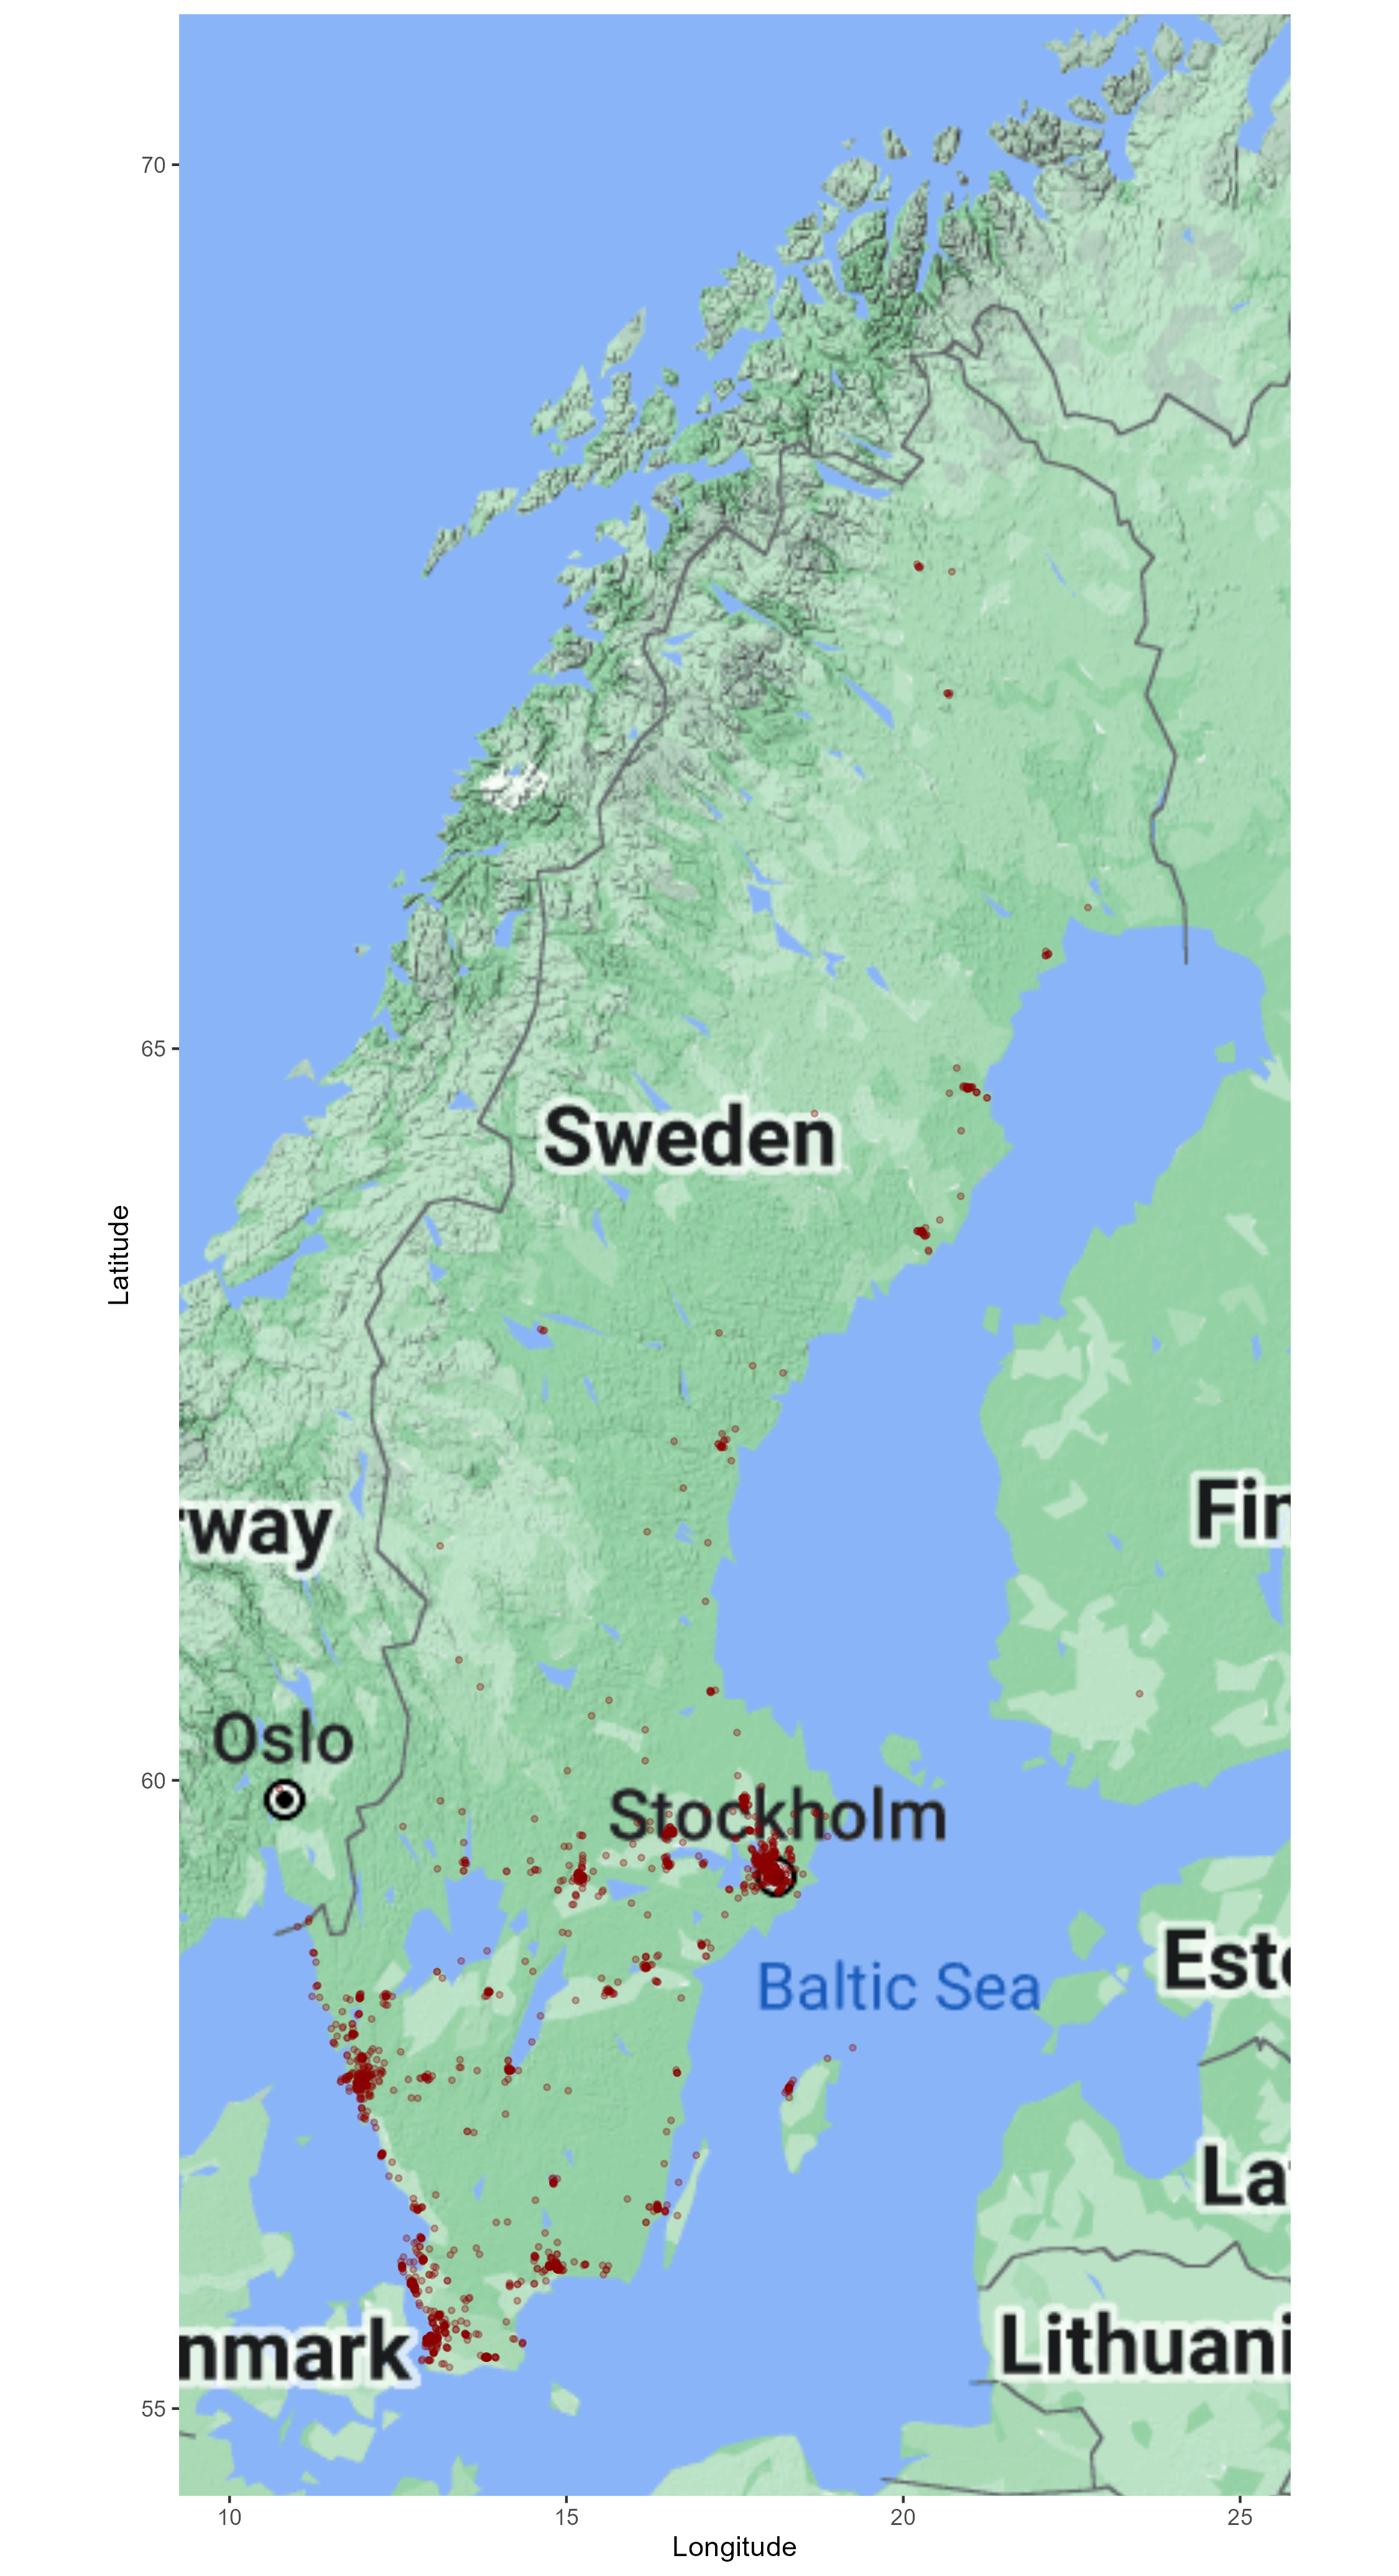
\includegraphics[scale=0.25]{figures/survey_location.png}
\caption{Country distribution of respondents \label{fig:map}}
\end{wrapfigure}
These housing companies included two local public housing providers and a national provider of tenant-owned dwellings, thereby representing various types of multi-family housing typically appealing to individuals from different socio-economic backgrounds.
\cite{caplanMeasuringHeterogeneousPreferences2021}

\subsection{Empirical design}

Stated choice experiments include a range of techniques in which respondents indicate their preferences by explicitly stating their choices. In contrast to revealed choice experiments, where preferences are inferred from past behaviour, stated choice methods allow for the evaluation of decisions in a controlled environment. This controlled setting enables the researcher to systematically manipulate attributes and isolate the impact of specific factors on decision-making. A Discrete Choice Experiment (DCE) is a popular type of stated choice model that presents individuals with hypothetical scenarios, allowing researchers to quantify how much value respondents place on different attributes of a product or service.

In our experiment,
respondents were asked to choose the most desirable housing option from a set of alternatives which contained varying levels of attributes.
Following standard practice,
the experiment instructed respondents to select a choice between two hypothetical housing scenarios in a particular choice set.
Each respondent was presented with a total of 9 choice sets,
where each choice set contained random attribute levels based on a D-optimality experimental design.

Careful attention was paid in designing and developing the experiment.

Next,
we present the attributes and their corresponding levels utilized in the experiment.


\subsection{Measurements of attributes}


The choice of attributes and associated levels in our study are a combination of important factors identified from the Prospective RELOC-AGE follow-up study and attributes found in the housing literature.
Following standard practice,
we select levels that allow for interpretability and viability of our willingness to pay estimates while holding certain attributes constant to make meaningful comparisons \citep{hensherAppliedChoiceAnalysis2015}.

Table \ref{tab:atts} shows the attributes selected and their associated levels.
The attribute \textit{greenspace} is defined as the distance in kilometres to green areas including parks, forests, hiking areas, and open spaces.
Similarly,
\textit{shops} represents the distance to shopping amenities such as grocery stores, malls, boutiques, and shopping centres.
The attribute \textit{transport} is the distance to transportation, such as a bus stop, metro station, or train station.
\textit{price} represents the percentage change in price the respondents for each alternative,
where monthly housing costs are known a priori from the initial questions on the survey.

Attributes were selected with to align with previous research as well as respondent answers from the follow-up Prospective RELOC-AGE survey.
Proximity to green areas has been examined in numerous contexts including improved cardiometabolic and general health \citep{paquetAreAccessibilityCharacteristics2013,  maasGreenSpaceUrbanity2006,},
lower stress \citep{nielsenGreenAreasAffect2007},
and improved mental health \citep{cohen-clineAccessGreenSpace2015,sturmProximityUrbanParks2014}.
Proximity to shops and services represent not only distance to frequent ammenities which may become more burndensome to transverse,
but also also may constitute an itergratl social experince to paricpate in the social live of communities
\citep{lucasMethodEvaluateEquitable2016}.
Distance to transportation has been shown to affect  accessibility levels of populations,
with significant differences identified in senior cohorts \citep{ricciardiExploringPublicTransport2015,hildebrandDimensionsElderlyTravel2003,alsnihMobilityAccessibilityExpectations2003}
Available parking facilities may also affect acceasability,
particularly for our sample where over 90\% of respondents indicated the have access to an automobile.
Taken together,
the literature offers extensive support in the importance of proximity to green areas, shops and services, and transportation.

Table \ref{tab:atts}  shows the attributes and their corresponding levels used in the experiment.


\begin{table}[H]
\scriptsize
\caption{Attributes and descriptions \label{tab:atts}}
\centering
\begin{tabular}[top]{>{\raggedright\arraybackslash}p{15em}l}
\toprule
Attribute & Description and levels\\
\midrule
Distance to green area & \makecell[l]{1 = within 500m \\ 2 = within 10km \\ 3 = within 15km}\\
\addlinespace
Distance to shops & \makecell[l]{1 = within 500m \\ 2 = within 10km \\ 3 = within 15km}\\
\addlinespace
Distance to public transportation & \makecell[l]{1 = within 300m \\ 2 = within 600 \\ 3 = within 900m}\\
\addlinespace
Parking & \makecell[l]{1 = no reserved parking \\ 2 = reserved parking place \\ 3 = reserved garage place}\\
\addlinespace
Price & \makecell[l]{1 = 20 \% less than planned costs \\ 2 = 10 \% less than planned costs \\ 3 = same as planned cost \\ 4 = 10 \% more than planned costs  \\ 5 = 20 \% more than planned costs}\\
\bottomrule
\end{tabular}
\end{table}



The number of choice sets is limited to 9 in order to minimize the cognitive burden of the DCE \citep{manghamHowNotDesigning2009,deshazoDesigningChoiceSets2002}
\footnote{\cite{himmlerWhatWorksBetter2021} highlights increased age would tend to exacerbated the cognitive burden of a discrete choice experiment, suggesting complex designs would lead to unreliable results.}.


Figure \ref{fig:choice_set} depicts a typical choice set presented to the respondents.
Before commencing the experiment,
respondents where given a definition of each attribute, as well as an example to clarify any ambiguity in interpretation of the attributes.
Respondents were also instructed to base each choice on the assumption that the alternative housing options where identical in every way aside from the attribute levels.


\begin{figure}[H]
\centering
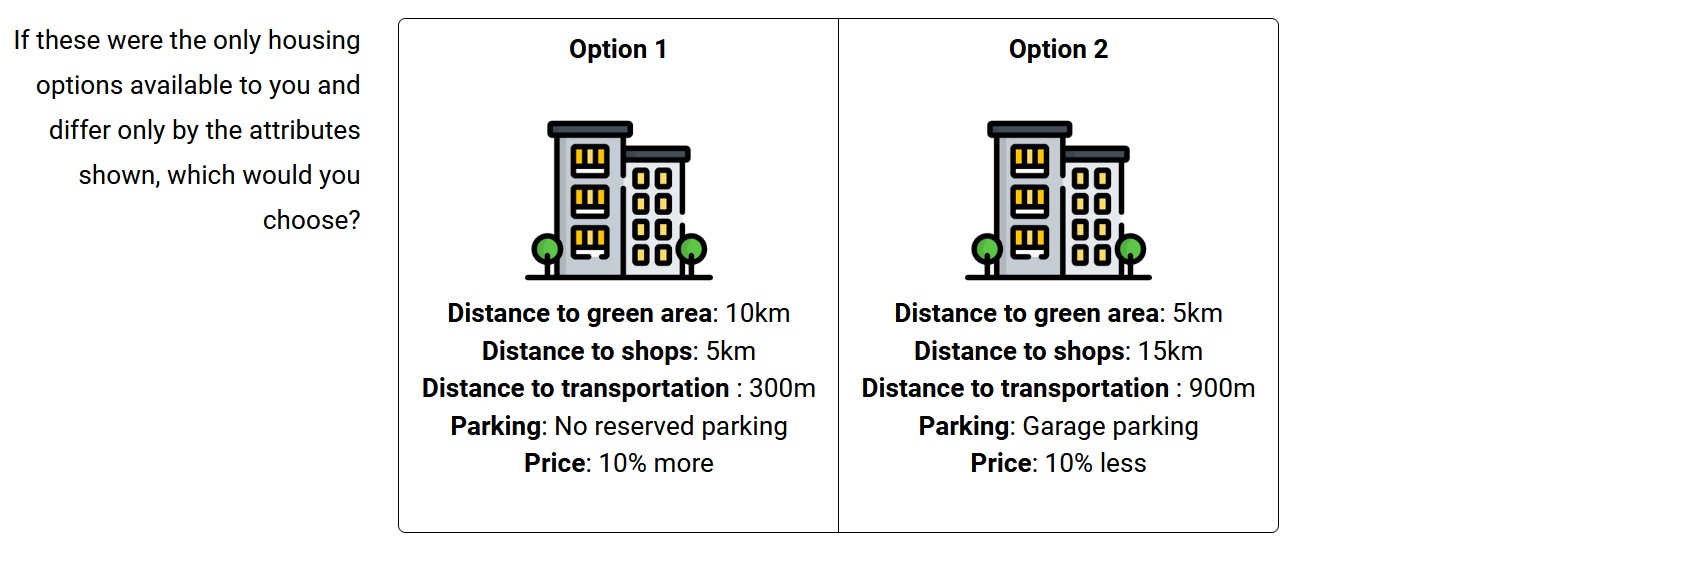
\includegraphics[scale=0.25]{figures/choice_set.png}
\caption{Example choice set \label{fig:choice_set}}
\end{figure}




%Despite the large amounts of attention these attributes have seen in the context of ageing and housing,
%knowledge gaps still remain.
%For instance,
%it is common that older individuals are examined as one homogeneous group in comparison to, for example, a younger cohort.
%This simplified grouping may miss key differences and shortcomings in interpretations.
%Importantly,
%this heterogeneity may be intensified throughout the population with the growth of the older population in the coming years.





%
%\cite{ricciardiExploringPublicTransport2015} "explore accessibility levels to public transport systems in the context of Perth, Australia, comparing seniors, low-income populations, populations without car availability, and the rest of the population. The findings reveal that the biggest accessibility differences are found in the seniors group, showing the lowest accessibility level to public transport systems."
%
%
%However, some studies have found significant differences within the senior cohort regarding travel behaviour and capacity to access certain locations.
%\cite{hildebrandDimensionsElderlyTravel2003}
%\cite{alsnihMobilityAccessibilityExpectations2003}

%\citep{lucasMethodEvaluateEquitable2016}. stress that physical grocery shopping may act as an integrated social experience.  Proximity to such shopping amenities can be crucial for older individuals to participate in the social life of their communities. 

%\cite{cohen-clineAccessGreenSpace2015} exaimine mental health and green areas among adult twin pairs, finding that greater access to green space is associated with less depression.
%
%In a Dutch study, \cite{maasGreenSpaceUrbanity2006} find that increased green space significantly reduces perceived general health, with elderly populations particularly benefiting more from the presence of green areas in their living environment.
%
%Using Danish survey data\cite{nielsenGreenAreasAffect2007} report results that indicate access to green areas are associtated with lower stress.
%
%\cite{paquetAreAccessibilityCharacteristics2013} report a relatinship between open spaces and better cardiometabolic health.
%
%
%\cite{sturmProximityUrbanParks2014} report findings that mental health is significantly related to residential distance from parks, suggesting mental health could be improved with enhanced environmental interventions. 











\clearpage





In a similar study,\cite{ossokinaBestLivingConcepts2020} 
run a discrete choice experiment utilizing predominately building characteristics in their model.

In the existing literature,
\cite{ossokinaReferencedependentHousingChoice2022a} is closest to our study in the choice of locational attributes.
The authors find that proximity to public transport has the highest effect on utility in their sample, followed by proximity to shops.
Our paper differs from theirs in a few ways.
First,
our sample is larger an encompasses a larger age group.
They have 441 home-owners in a nine year age group (65-75).
Second,
our study comprises both home owners and rental occupants, representing a larger diversity of individuals searching for housing.
Finally,
instead of a purely hypothetical experimnet, the respondents in our study have signed up for housing services, where we can assume they have the intention, or at least a strong consideration, to relocate.







\newpage

\section{Methods}

\subsection{Survey development and design}




Survey was hosted on university servers and implimented in the open source survey framework formr.


The choice experiment was administered in conjunction with the second follow-up survey in January 2024,
where 1,297 of the 1,952 original respondents agreed to participate in the experiment.
Respondents who had already relocated and those who did not fully complete the survey questions were excluded, leading to a final sample size of 957 individuals.
The experiment was administered within the flexible survey framework Formr and open to participating respondents from 

Table \ref{tab:des} presents the results.
Among the sample, 55\% were female, 46\% were male, and the majority (64\%) reported being married or cohabiting with a partner. Additionally, 73\% of respondents fell within the age range of 54-74, and the majority rated their health as either good (34\%) or very good (33\%).

\begin{table}


%\begin{wraptable}{r}{0.4\textwidth} 
\begin{table}[h]
\centering
\caption{Descriptive statistics}
\label{tab:desc}
\begin{threeparttable}
\begin{tabular}{lccc}
\scriptsize
\toprule
 & \textbf{Owner (N=790)} & \textbf{Renter (N=167)} & \textbf{Overall (N=957)} \\
\midrule
\textbf{Sex} \\
\hspace{1em}Female & 419 (53.0\%) & 110 (65.9\%) & 529 (55.3\%) \\
\hspace{1em}Male & 371 (47.0\%) & 57 (34.1\%) & 428 (44.7\%) \\

\textbf{Age group} \\
\hspace{1em}55--64 & 154 (19.5\%) & 38 (22.8\%) & 192 (20.1\%) \\
\hspace{1em}65--74 & 344 (43.5\%) & 72 (43.1\%) & 416 (43.5\%) \\
\hspace{1em}75+ & 292 (37.0\%) & 57 (34.1\%) & 349 (36.5\%) \\

\textbf{Civil status} \\
\hspace{1em}Not partnered & 287 (36.3\%) & 90 (53.9\%) & 377 (39.4\%) \\
\hspace{1em}Partnered & 503 (63.7\%) & 77 (46.1\%) & 580 (60.6\%) \\

\textbf{Retired} \\
\hspace{1em}Yes & 612 (77.5\%) & 126 (75.4\%) & 738 (77.1\%) \\
\hspace{1em}No & 174 (22.0\%) & 41 (24.6\%) & 215 (22.5\%) \\
\hspace{1em}Missing & 4 (0.5\%) & 0 (0.0\%) & 4 (0.4\%) \\

\textbf{Current housing type} \\
\hspace{1em}Apartment/Condo & 447 (56.6\%) & 153 (91.6\%) & 600 (62.7\%) \\
\hspace{1em}House & 341 (43.2\%) & 13 (7.8\%) & 354 (37.0\%) \\
\hspace{1em}Missing & 2 (0.3\%) & 1 (0.6\%) & 3 (0.3\%) \\

\textbf{Current housing location} \\
\hspace{1em}City/town & 478 (60.5\%) & 117 (70.1\%) & 595 (62.2\%) \\
\hspace{1em}Urban area & 221 (28.0\%) & 41 (24.6\%) & 262 (27.4\%) \\
\hspace{1em}Countryside & 81 (10.3\%) & 6 (3.6\%) & 87 (9.1\%) \\
\hspace{1em}Missing & 10 (1.3\%) & 3 (1.8\%) & 13 (1.4\%) \\

\textbf{Monthly household income} \\
\hspace{1em}Mean (SD) & 48700 (34700) & 37700 (27900) & 46700 (33900) \\
\hspace{1em}Median [Min, Max] & 44300 [0, 220000] & 35000 [0, 153000] & 40500 [0, 220000] \\
\hspace{1em}Missing & 6 (0.8\%) & 0 (0.0\%) & 6 (0.6\%) \\

\textbf{Planned housing costs} \\
\hspace{1em}Mean (SD) & 10400 (4060) & 10500 (5570) & 10500 (4370) \\
\hspace{1em}Median [Min, Max] & 10000 [3000, 40000] & 9000 [3000, 60000] & 10000 [3000, 60000] \\
\hspace{1em}Missing & 95 (12.0\%) & 15 (9.0\%) & 110 (11.5\%) \\
\bottomrule
\end{tabular}
\end{threeparttable}
\end{table}

%\end{wraptable}

\end{table}




\subsection{Empirical Models}

Utilizing the discrete choice data,
respondent's choices may be modelled within a random utility theory framework,
which assumes individuals choose options which maximize an underlying utility model\citep{lancsarConductingDiscreteChoice2008}.
Under the random utility theory framework, the utility that individual \( i \) derives from alternative \( j \) in a choice set \( t \) is given by:

\begin{equation}
U_{ijt} = V_{ijt} + \varepsilon_{ijt}
\end{equation}

\noindent where \( V_{ijt} \) is the systematic component of utility, modelled as a function of the attributes of the alternative, and \( \varepsilon_{ijt} \) is the unobserved random error term.
The systematic utility is specified as:

\begin{equation}
V_{ijt} = \beta_1 X_{ijt1} + \beta_2 X_{ijt2} + \ldots + \beta_k X_{ijtk}
\end{equation}

\noindent where \( X_{ijtk} \) represents the level of attribute \( k \) for alternative \( j \) in task \( t \), and \( \beta_k \) are the corresponding utility coefficients to be estimated.
In other words,
these \( X_{ijtk} \) represent the respective attributes found in \ref{tab:atts}.



We estimate both multinomial logit (MNL) models and a mixed logit (ML) models in our testing.
The MNL model assumes homogeneous preferences across respondents and independently and identically distributed (i.i.d.) error terms.
Choice probabilities are given by the standard logit formula:

\begin{equation}
P_{ijt} = \frac{\exp(V_{ijt})}{\sum_{l=1}^{J} \exp(V_{ilt})}
\end{equation}

To account for unobserved heterogeneity in preferences, we estimate a mixed logit model, in which the utility coefficients \( \boldsymbol{\beta}_i \) are allowed to vary randomly across individuals \citep{mcfaddenMixedMNLModels2000}:

\begin{equation}
\boldsymbol{\beta}_i = \boldsymbol{\beta} + \Sigma \eta_i
\end{equation}

\noindent where \( \eta_i \sim \mathcal{N}(0, I) \) and \( \Sigma \) is the covariance matrix of the random parameters. The mixed logit model captures heterogeneity by integrating over the distribution of random coefficients using simulated maximum likelihood.

We use our price attribute to compute monetary trade-offs for non-cost attributes. 
First,
we estimate marginal rate of substitution (MRS) for each attribute,
where the MRS for attribute \( k \) is calculated as:

\begin{equation}
\text{MRS}_k = -\frac{\hat{\beta}_k}{\hat{\beta}_{\text{cost}}}
\end{equation}

\noindent where \( \hat{\beta}_{\text{cost}} \) is the estimated coefficient on the cost attribute.

To convert the MRS into marginal willingness to pay (MWTP) in SEK, we multiply by 10 percent of the mean planned monthly housing cost reported by respondents:

\begin{equation}
\text{MWTP}_k = \text{MRS}_k \times 0.10 \times \bar{C}
\end{equation}

\noindent where \( \bar{C} \) is the sample mean of respondents' stated planned monthly housing cost.

These MWTP values represent how much, in SEK per month, respondents are willing to pay for improvements in each housing attribute, relative to their housing cost expectations. This enables direct comparison of attribute valuations across different socio-demographic groups and tenure types.

\subsection{Estimation and Software}

All models are estimated in R using the \texttt{logitr} package \citep{helvestonLogitrFastEstimation2022}, which provides flexible estimation routines for both MNL and MXL models using simulated maximum likelihood. For the MXL models, we use Halton draws to simulate the integrals over random parameters, and we cluster standard errors at the individual level to account for repeated observations per respondent.




\subsection{Willingness to pay}
Marginal willingness to pay for attribute $k$ is computed as the ratio of the attribute coefficient to the cost coefficient:
\begin{equation}
\text{MWTP}_{k,i} \;=\; - \frac{\beta_{k,i}}{\beta_{p,i}}.
\end{equation}
We report mean and percentile summaries of the implied MWTP distribution using the simulated draws of $\beta_{k,i}$ and $\beta_{p,i}$, along with delta method or simulation based standard errors. Because the cost attribute is specified as a percentage change, we convert MWTP to monetary terms by scaling with each respondent's reported or imputed baseline housing cost, consistent with \citet{Caplan2021}.




\section{Empirical Results}


Our discussion begins with results from the baseline model, which excludes interaction terms and serves as a point of comparison for subsequent models that account for heterogeneity across household types.
Table \ref{tab:base_owner} presents the estimation results for respondents who own their housing unit.
In this specification, a positive (negative) coefficient indicates an increase (decrease) in average utility associated with the attribute level, relative to its reference category. We report coefficient estimates from the multinomial logit model in column two and from the mixed logit model in column three.
Results from both models are included to facilitate comparison and to assess the robustness of the findings across model specifications.


\begin{table}[h]
\caption{Baseline results - Owner}
\label{tab:base_owner}
\begin{center}
\scriptsize
\begin{tabular}{l D{.}{.}{5.5} D{.}{.}{5.5} D{.}{.}{2.5} D{.}{.}{2.5} D{.}{.}{3.2}}
\toprule
 & & \multicolumn{2}{c}{MXL} \\
\cmidrule(lr){3-4}
 & \multicolumn{1}{c}{MNL} & \multicolumn{1}{c}{Mean} & \multicolumn{1}{c}{SD} & \multicolumn{1}{c}{MRS} & \multicolumn{1}{c}{MWTP (SEK/mo)} \\
\midrule
Green space: 5 km (vs 15 km)       & 0.57^{***}  & 1.16^{***}  & 0.12        & 0.22^{***} & 232.29 \\
                                   & (0.05)      & (0.12)      & (0.23)      & (0.02)     &        \\
Green space: 500 m (vs 15 km)      & 1.12^{***}  & 2.21^{***}  & 1.24^{***}  & 0.42^{***} & 440.66 \\
                                   & (0.05)      & (0.16)      & (0.25)      & (0.03)     &        \\
Shops: 5 km (vs 15 km)             & 0.58^{***}  & 1.01^{***}  & 0.10        & 0.19^{***} & 200.82 \\
                                   & (0.05)      & (0.13)      & (0.20)      & (0.03)     &        \\
Shops: 500 m (vs 15 km)            & 1.68^{***}  & 3.12^{***}  & 1.05^{***}  & 0.59^{***} & 622.34 \\
                                   & (0.05)      & (0.18)      & (0.21)      & (0.04)     &        \\
Transit stop: 600 m (vs 900 m)     & 0.20^{***}  & 0.35^{**}   & -0.76^{***} & 0.07^{**}  & 69.56  \\
                                   & (0.05)      & (0.11)      & (0.20)      & (0.02)     &        \\
Transit stop: 300 m (vs 900 m)     & 0.51^{***}  & 1.13^{***}  & 0.79^{***}  & 0.21^{***} & 225.03 \\
                                   & (0.05)      & (0.12)      & (0.18)      & (0.02)     &        \\
Parking: reserved garage (vs none) & 1.53^{***}  & 3.08^{***}  & 0.56^{*}    & 0.59^{***} & 615.13 \\
                                   & (0.06)      & (0.20)      & (0.25)      & (0.04)     &        \\
Parking: reserved space (vs none)  & 1.30^{***}  & 2.56^{***}  & -2.29^{***} & 0.49^{***} & 511.17 \\
                                   & (0.06)      & (0.17)      & (0.17)      & (0.03)     &        \\
Price                              & -2.83^{***} & -5.26^{***} &             &            &        \\
                                   & (0.16)      & (0.35)      &             &            &        \\
\midrule
Num. obs.                          & 7110        & 7110        &             &            &        \\
Log Likelihood                     & -3570.76    & -3136.51    &             &            &        \\
AIC                                & 7159.53     & 6363.02     &             &            &        \\
BIC                                & 7221.35     & 6672.14     &             &            &        \\
McFadden R²                        & 0.28        & 0.36        &             &            &        \\
LR \chi 2 (df=9)                       & 2715.02     & 3583.53     &             &            &        \\
p-value (LR)                       & 0.00        & 0.00        &             &            &        \\
\bottomrule
\multicolumn{6}{l}{\scriptsize{$^{***}p<0.001$; $^{**}p<0.01$; $^{*}p<0.05$}}
\end{tabular}
\end{center}
\end{table}



Although both model specifications yield similar patterns in coefficient signs and levels of statistical significance, the mixed logit estimates (column three) are systematically larger in magnitude than those from the multinomial logit model.
In terms of model performance, the mixed logit specification demonstrates superior fit across all criteria, including log-likelihood, McFadden's pseudo-R2, AIC, and BIC.
Additionally, several standard deviation estimates for the random parameters (column four) are statistically significant, confirming the presence of preference heterogeneity for certain attributes.
We therefore adopt the mixed logit specification as our preferred model for all subsequent interpretation and discussion.

Marginal rate of substitution (MRS) estimates are presented in column five and are calculated as described in Equation (XX). To obtain marginal willingness to pay (MWTP) estimates, MRS values are multiplied by 10 percent of each respondent's reported planned housing cost, following Equation (YY). These monetary estimates are presented in column six.

As shown in Table~\ref{tab:base_owner},
owners are, on average, willing to pay up to 440 SEK per month to avoid residing 15 kilometers from the nearest green area. Proximity to shops appears to be even more highly valued, with owners willing to pay over 620 SEK per month to avoid similar distance from retail services.

Table~\ref{tab:base_renter} presents results for respondents who do not own their current housing. Compared to owners, renters place even higher value on proximity to green space, with an estimated MWTP that is 177 SEK greater. Renters also value proximity to shops more highly, with an average MWTP of 636 SEK for locations within 500 meters, compared to 622 SEK for owners.

Reserved parking emerges as a critical attribute across both tenure groups. However, owners are willing to pay substantially more for access to a reserved garage (615 SEK vs 337 SEK),
suggesting stronger preferences for secure or private vehicle storage among this group.


\begin{table}[h]
\caption{Baseline results - Renter}
\label{tab:base_renter}
\begin{center}
\scriptsize
\begin{tabular}{l D{.}{.}{4.5} D{.}{.}{4.5} D{.}{.}{2.5} D{.}{.}{2.5} D{.}{.}{3.2}}
\toprule
 & & \multicolumn{2}{c}{MXL} \\
\cmidrule(lr){3-4}
 & \multicolumn{1}{c}{MNL} & \multicolumn{1}{c}{Mean} & \multicolumn{1}{c}{SD} & \multicolumn{1}{c}{MRS} & \multicolumn{1}{c}{MWTP (SEK/mo)} \\
\midrule
Green space: 5 km (vs 15 km)       & 0.75^{***}  & 4.80^{***}   & 2.30^{***}  & 0.36^{***} & 377.54 \\
                                   & (0.11)      & (1.29)       & (0.65)      & (0.06)     &        \\
Green space: 500 m (vs 15 km)      & 1.25^{***}  & 7.85^{***}   & 6.64^{***}  & 0.59^{***} & 618.10 \\
                                   & (0.12)      & (2.07)       & (1.85)      & (0.08)     &        \\
Shops: 5 km (vs 15 km)             & 0.77^{***}  & 3.67^{**}    & 0.36        & 0.27^{***} & 288.71 \\
                                   & (0.12)      & (1.15)       & (0.46)      & (0.06)     &        \\
Shops: 500 m (vs 15 km)            & 1.68^{***}  & 8.09^{***}   & 6.47^{***}  & 0.61^{***} & 636.95 \\
                                   & (0.12)      & (2.12)       & (1.81)      & (0.09)     &        \\
Transit stop: 600 m (vs 900 m)     & 0.30^{*}    & 1.57^{**}    & 0.99        & 0.12^{**}  & 123.73 \\
                                   & (0.12)      & (0.55)       & (0.63)      & (0.04)     &        \\
Transit stop: 300 m (vs 900 m)     & 0.68^{***}  & 2.01^{***}   & 1.64^{**}   & 0.15^{***} & 158.21 \\
                                   & (0.12)      & (0.52)       & (0.57)      & (0.03)     &        \\
Parking: reserved garage (vs none) & 0.92^{***}  & 4.28^{***}   & -0.02       & 0.32^{***} & 337.04 \\
                                   & (0.12)      & (0.97)       & (0.32)      & (0.04)     &        \\
Parking: reserved space (vs none)  & 0.94^{***}  & 3.90^{***}   & -4.64^{***} & 0.29^{***} & 306.98 \\
                                   & (0.13)      & (0.82)       & (1.35)      & (0.03)     &        \\
Price                              & -4.10^{***} & -13.34^{***} &             &            &        \\
                                   & (0.37)      & (2.61)       &             &            &        \\
\midrule
Num. obs.                          & 1458        & 1458         &             &            &        \\
Log Likelihood                     & -721.69     & -612.41      &             &            &        \\
AIC                                & 1461.39     & 1314.82      &             &            &        \\
BIC                                & 1508.95     & 1552.64      &             &            &        \\
McFadden R²                        & 0.29        & 0.39         &             &            &        \\
LR $\chi 2$ (df=9)                       & 577.83      & 796.40       &             &            &        \\
p-value (LR)                       & 0.00        & 0.00         &             &            &        \\
\bottomrule
\multicolumn{6}{l}{\scriptsize{$^{***}p<0.001$; $^{**}p<0.01$; $^{*}p<0.05$}}
\end{tabular}
\end{center}
\end{table}





\begin{table}[h]
\caption{Baseline results - Male}
\label{table:base_male}
\begin{center}
\scriptsize
\begin{tabular}{l D{.}{.}{5.5} D{.}{.}{5.5} D{.}{.}{2.5} D{.}{.}{2.5} D{.}{.}{3.2}}
\toprule
 & & \multicolumn{2}{c}{MXL} \\
\cmidrule(lr){3-4}
 & \multicolumn{1}{c}{MNL} & \multicolumn{1}{c}{Mean} & \multicolumn{1}{c}{SD} & \multicolumn{1}{c}{MRS} & \multicolumn{1}{c}{MWTP (SEK/mo)} \\
\midrule
Green space: 5 km (vs 15 km)       & 0.65^{***}  & 1.33^{***}  & -0.25       & 0.23^{***} & 227.78 \\
                                   & (0.07)      & (0.16)      & (0.24)      & (0.03)     &        \\
Green space: 500 m (vs 15 km)      & 1.01^{***}  & 2.05^{***}  & 1.16^{***}  & 0.35^{***} & 351.54 \\
                                   & (0.07)      & (0.20)      & (0.32)      & (0.04)     &        \\
Shops: 5 km (vs 15 km)             & 0.69^{***}  & 1.26^{***}  & 0.32        & 0.22^{***} & 215.57 \\
                                   & (0.08)      & (0.18)      & (0.26)      & (0.04)     &        \\
Shops: 500 m (vs 15 km)            & 1.76^{***}  & 3.45^{***}  & 0.17        & 0.59^{***} & 590.67 \\
                                   & (0.07)      & (0.25)      & (0.30)      & (0.05)     &        \\
Transit stop: 600 m (vs 900 m)     & 0.20^{**}   & 0.32^{*}    & -1.14^{***} & 0.05       & 54.05  \\
                                   & (0.08)      & (0.16)      & (0.23)      & (0.03)     &        \\
Transit stop: 300 m (vs 900 m)     & 0.41^{***}  & 0.85^{***}  & 0.21        & 0.15^{***} & 145.00 \\
                                   & (0.07)      & (0.16)      & (0.20)      & (0.03)     &        \\
Parking: reserved garage (vs none) & 1.71^{***}  & 3.65^{***}  & -1.54^{***} & 0.62^{***} & 624.07 \\
                                   & (0.08)      & (0.29)      & (0.24)      & (0.05)     &        \\
Parking: reserved space (vs none)  & 1.43^{***}  & 3.12^{***}  & 2.66^{***}  & 0.53^{***} & 533.73 \\
                                   & (0.08)      & (0.26)      & (0.25)      & (0.04)     &        \\
Price                              & -3.01^{***} & -5.84^{***} &  -          &  -         &  -     \\
                                   & (0.22)      & (0.52)      &             &            &        \\
\midrule
Num. obs.                          & 3852        & 3852        &             & -          &  -     \\
Log Likelihood                     & -1889.12    & -1648.41    &             & -          &  -     \\
AIC                                & 3796.25     & 3386.81     &             & -          &  -     \\
BIC                                & 3852.55     & 3668.35     &             & -          &  -     \\
McFadden R²                        & 0.29        & 0.38        &             & -          &  -     \\
LR χ² (df=9)                       & 1561.76     & 2043.19     &             & -          &  -     \\
p-value (LR)                       & 0.00        & 0.00        &             & -          &  -     \\
\bottomrule
\multicolumn{6}{l}{\scriptsize{$^{***}p<0.001$; $^{**}p<0.01$; $^{*}p<0.05$}}
\end{tabular}

\end{center}
\end{table}


\begin{table}[h]
\caption{Baseline results - Female}
\label{table:base_male}
\begin{center}
\scriptsize
\begin{tabular}{l D{.}{.}{5.5} D{.}{.}{5.5} D{.}{.}{2.5} D{.}{.}{2.5} D{.}{.}{3.2}}
\toprule
 & & \multicolumn{2}{c}{MXL} \\
\cmidrule(lr){3-4}
 & \multicolumn{1}{c}{MNL} & \multicolumn{1}{c}{Mean} & \multicolumn{1}{c}{SD} & \multicolumn{1}{c}{MRS} & \multicolumn{1}{c}{MWTP (SEK/mo)} \\
\midrule
Green space: 5 km (vs 15 km)       & 0.56^{***}  & 1.25^{***}  & 0.25        & 0.23^{***} & 242.97 \\
                                   & (0.06)      & (0.17)      & (0.54)      & (0.03)     &        \\
Green space: 500 m (vs 15 km)      & 1.24^{***}  & 2.76^{***}  & 1.24^{**}   & 0.51^{***} & 537.22 \\
                                   & (0.06)      & (0.24)      & (0.43)      & (0.05)     &        \\
Shops: 5 km (vs 15 km)             & 0.55^{***}  & 1.07^{***}  & 0.86^{**}   & 0.20^{***} & 207.50 \\
                                   & (0.06)      & (0.21)      & (0.29)      & (0.04)     &        \\
Shops: 500 m (vs 15 km)            & 1.61^{***}  & 3.10^{***}  & 1.33^{***}  & 0.57^{***} & 602.77 \\
                                   & (0.06)      & (0.24)      & (0.39)      & (0.05)     &        \\
Transit stop: 600 m (vs 900 m)     & 0.24^{***}  & 0.50^{***}  & -0.09       & 0.09^{***} & 98.21  \\
                                   & (0.07)      & (0.14)      & (0.32)      & (0.03)     &        \\
Transit stop: 300 m (vs 900 m)     & 0.65^{***}  & 1.38^{***}  & 1.03^{***}  & 0.26^{***} & 268.90 \\
                                   & (0.06)      & (0.16)      & (0.22)      & (0.03)     &        \\
Parking: reserved garage (vs none) & 1.21^{***}  & 2.43^{***}  & 0.41        & 0.45^{***} & 473.25 \\
                                   & (0.07)      & (0.20)      & (0.26)      & (0.04)     &        \\
Parking: reserved space (vs none)  & 1.10^{***}  & 1.96^{***}  & -2.17^{***} & 0.36^{***} & 381.55 \\
                                   & (0.07)      & (0.18)      & (0.25)      & (0.03)     &        \\
Price                              & -3.07^{***} & -5.40^{***} &             &            &        \\
                                   & (0.19)      & (0.44)      &             &            &        \\
\midrule
Num. obs.                          & 4761        & 4761        &             &            &        \\
Log Likelihood                     & -2431.00    & -2122.98    &             &            &        \\
AIC                                & 4880.00     & 4335.96     &             &            &        \\
BIC                                & 4938.21     & 4627.03     &             &            &        \\
McFadden R²                        & 0.26        & 0.36        &             &            &        \\
LR \chi 2 (df=9)                       & 1738.15     & 2354.18     &             &            &        \\
p-value (LR)                       & 0.00        & 0.00        &             &            &        \\
\bottomrule
\multicolumn{6}{l}{\scriptsize{$^{***}p<0.001$; $^{**}p<0.01$; $^{*}p<0.05$}}
\end{tabular}
\end{center}
\end{table}



\begin{table}
\caption{Baseline results - 55-64}
\begin{center}
\begin{scriptsize}
\begin{tabular}{l D{.}{.}{4.5} D{.}{.}{4.5} D{.}{.}{2.5} D{.}{.}{2.5} D{.}{.}{3.2}}
\toprule
 & & \multicolumn{2}{c}{ML} \\
\cmidrule(lr){3-4}
 & \multicolumn{1}{c}{MNL} & \multicolumn{1}{c}{Mean} & \multicolumn{1}{c}{SD} & \multicolumn{1}{c}{MRS} & \multicolumn{1}{c}{MWTP} \\
\midrule
Green space: 5 km (vs 15 km)       & 0.63^{***}  & 1.95^{***}   & -0.63       & 0.19^{***} & 200.97 \\
                                   & (0.10)      & (0.40)       & (0.48)      & (0.03)     &        \\
Green space: 500 m (vs 15 km)      & 1.45^{***}  & 4.81^{***}   & 4.35^{***}  & 0.47^{***} & 495.74 \\
                                   & (0.11)      & (0.73)       & (0.82)      & (0.05)     &        \\
Shops: 5 km (vs 15 km)             & 0.65^{***}  & 1.67^{***}   & 0.40        & 0.16^{***} & 172.18 \\
                                   & (0.12)      & (0.41)       & (0.39)      & (0.04)     &        \\
Shops: 500 m (vs 15 km)            & 1.76^{***}  & 4.94^{***}   & 1.07^{*}    & 0.48^{***} & 509.16 \\
                                   & (0.11)      & (0.65)       & (0.44)      & (0.05)     &        \\
Transit stop: 600 m (vs 900 m)     & 0.10        & 0.59         & 1.90^{***}  & 0.06       & 60.54  \\
                                   & (0.11)      & (0.33)       & (0.44)      & (0.03)     &        \\
Transit stop: 300 m (vs 900 m)     & 0.60^{***}  & 1.89^{***}   & -0.08       & 0.19^{***} & 194.66 \\
                                   & (0.11)      & (0.38)       & (0.47)      & (0.03)     &        \\
Parking: reserved garage (vs none) & 1.31^{***}  & 3.84^{***}   & -1.66^{***} & 0.38^{***} & 395.29 \\
                                   & (0.11)      & (0.68)       & (0.45)      & (0.05)     &        \\
Parking: reserved space (vs none)  & 1.04^{***}  & 3.19^{***}   & 3.84^{***}  & 0.31^{***} & 328.33 \\
                                   & (0.12)      & (0.54)       & (0.70)      & (0.04)     &        \\
Price                              & -3.99^{***} & -10.19^{***} &             &            &        \\
                                   & (0.36)      & (1.42)       &             &            &        \\
\midrule
Num. obs.                          & 1728        & 1728         &             &            &        \\
Log Likelihood                     & -817.95     & -689.10      &             &            &        \\
AIC                                & 1653.91     & 1468.20      &             &            &        \\
BIC                                & 1703.00     & 1713.66      &             &            &        \\
McFadden R²                        & 0.32        & 0.42         &             &            &        \\
LR $\chi 2$ (df=9)                       & 759.61      & 1017.32      &             &            &        \\
p-value (LR)                       & 0.00        & 0.00         &             &            &        \\
\bottomrule
\multicolumn{6}{l}{\tiny{$^{***}p<0.001$; $^{**}p<0.01$; $^{*}p<0.05$}}
\end{tabular}
\end{scriptsize}
\label{table:55_64}
\end{center}
\end{table}


\begin{table}
\caption{Mixed Logit Estimates for 65-74 : Base Specification}
\begin{center}
\begin{scriptsize}
\begin{tabular}{l D{.}{.}{5.5} D{.}{.}{5.5} D{.}{.}{2.5} D{.}{.}{2.5} D{.}{.}{3.2}}
\toprule
 & & \multicolumn{2}{c}{MXL} \\
\cmidrule(lr){3-4}
 & \multicolumn{1}{c}{MNL} & \multicolumn{1}{c}{Mean} & \multicolumn{1}{c}{SD} & \multicolumn{1}{c}{MRS} & \multicolumn{1}{c}{MWTP (SEK/mo)} \\
\midrule
Green space: 5 km (vs 15 km)       & 0.62^{***}  & 1.38^{***}  & 0.38       & 0.20^{***} & 214.30 \\
                                   & (0.07)      & (0.22)      & (0.24)     & (0.03)     &        \\
Green space: 500 m (vs 15 km)      & 1.18^{***}  & 2.66^{***}  & 0.53       & 0.39^{***} & 411.97 \\
                                   & (0.07)      & (0.33)      & (0.40)     & (0.04)     &        \\
Shops: 5 km (vs 15 km)             & 0.54^{***}  & 1.05^{***}  & 0.52       & 0.16^{***} & 163.48 \\
                                   & (0.07)      & (0.24)      & (0.38)     & (0.04)     &        \\
Shops: 500 m (vs 15 km)            & 1.70^{***}  & 3.72^{***}  & 2.22^{***} & 0.55^{***} & 576.94 \\
                                   & (0.08)      & (0.39)      & (0.29)     & (0.05)     &        \\
Transit stop: 600 m (vs 900 m)     & 0.20^{**}   & 0.24        & -0.67^{**} & 0.04       & 36.99  \\
                                   & (0.08)      & (0.16)      & (0.24)     & (0.02)     &        \\
Transit stop: 300 m (vs 900 m)     & 0.54^{***}  & 1.10^{***}  & 1.19^{***} & 0.16^{***} & 170.35 \\
                                   & (0.07)      & (0.19)      & (0.25)     & (0.03)     &        \\
Parking: reserved garage (vs none) & 1.51^{***}  & 3.61^{***}  & 1.08^{***} & 0.53^{***} & 559.50 \\
                                   & (0.08)      & (0.37)      & (0.25)     & (0.05)     &        \\
Parking: reserved space (vs none)  & 1.26^{***}  & 2.69^{***}  & 2.55^{***} & 0.40^{***} & 416.65 \\
                                   & (0.08)      & (0.28)      & (0.38)     & (0.03)     &        \\
Price                              & -3.09^{***} & -6.77^{***} &            &            &        \\
                                   & (0.22)      & (0.65)      &            &            &        \\
\midrule
Num. obs.                          & 3744        & 3744        &            &            &        \\
Log Likelihood                     & -1868.23    & -1646.37    &            &            &        \\
AIC                                & 3754.45     & 3382.73     &            &            &        \\
BIC                                & 3810.50     & 3662.99     &            &            &        \\
McFadden R²                        & 0.28        & 0.37        &            &            &        \\
LR χ² (df=9)                       & 1453.83     & 1897.56     &            &            &        \\
p-value (LR)                       & 0.00        & 0.00        &            &            &        \\
\bottomrule
\multicolumn{6}{l}{\tiny{$^{***}p<0.001$; $^{**}p<0.01$; $^{*}p<0.05$}}
\end{tabular}
\end{scriptsize}
\label{table:coefficients}
\end{center}
\end{table}


\begin{table}
\caption{Mixed Logit Estimates for 75+ : Base Specification}
\begin{center}
\begin{scriptsize}
\begin{tabular}{l D{.}{.}{5.5} D{.}{.}{5.5} D{.}{.}{2.5} D{.}{.}{2.5} D{.}{.}{3.2}}
\toprule
 & & \multicolumn{2}{c}{MXL} \\
\cmidrule(lr){3-4}
 & \multicolumn{1}{c}{MNL} & \multicolumn{1}{c}{Mean} & \multicolumn{1}{c}{SD} & \multicolumn{1}{c}{MRS} & \multicolumn{1}{c}{MWTP (SEK/mo)} \\
\midrule
Green space: 5 km (vs 15 km)       & 0.55^{***}  & 1.10^{***}  & -0.17       & 0.23^{***} & 238.16 \\
                                   & (0.07)      & (0.21)      & (0.28)      & (0.05)     &        \\
Green space: 500 m (vs 15 km)      & 0.95^{***}  & 2.01^{***}  & 0.40        & 0.41^{***} & 434.70 \\
                                   & (0.08)      & (0.25)      & (0.36)      & (0.06)     &        \\
Shops: 5 km (vs 15 km)             & 0.66^{***}  & 1.21^{***}  & 0.47        & 0.25^{***} & 261.18 \\
                                   & (0.08)      & (0.22)      & (0.28)      & (0.06)     &        \\
Shops: 500 m (vs 15 km)            & 1.59^{***}  & 3.34^{***}  & 0.13        & 0.69^{***} & 722.79 \\
                                   & (0.08)      & (0.33)      & (0.25)      & (0.08)     &        \\
Transit stop: 600 m (vs 900 m)     & 0.32^{***}  & 0.55^{***}  & -0.70^{***} & 0.11^{**}  & 119.57 \\
                                   & (0.08)      & (0.16)      & (0.21)      & (0.04)     &        \\
Transit stop: 300 m (vs 900 m)     & 0.52^{***}  & 1.20^{***}  & 0.57^{*}    & 0.25^{***} & 258.91 \\
                                   & (0.08)      & (0.20)      & (0.25)      & (0.04)     &        \\
Parking: reserved garage (vs none) & 1.42^{***}  & 3.04^{***}  & 0.61^{*}    & 0.63^{***} & 658.01 \\
                                   & (0.08)      & (0.29)      & (0.24)      & (0.08)     &        \\
Parking: reserved space (vs none)  & 1.33^{***}  & 2.76^{***}  & -2.61^{***} & 0.57^{***} & 597.03 \\
                                   & (0.09)      & (0.26)      & (0.31)      & (0.06)     &        \\
Price                              & -2.51^{***} & -4.86^{***} &             &            &        \\
                                   & (0.23)      & (0.55)      &             &            &        \\
\midrule
Num. obs.                          & 3141        & 3141        &             &            &        \\
Log Likelihood                     & -1632.69    & -1425.97    &             &            &        \\
AIC                                & 3283.38     & 2941.93     &             &            &        \\
BIC                                & 3337.85     & 3214.29     &             &            &        \\
McFadden R²                        & 0.25        & 0.35        &             &            &        \\
LR $\chi 2$ (df=9)                       & 1088.97     & 1502.42     &             &            &        \\
p-value (LR)                       & 0.00        & 0.00        &             &            &        \\
\bottomrule
\multicolumn{6}{l}{\tiny{$^{***}p<0.001$; $^{**}p<0.01$; $^{*}p<0.05$}}
\end{tabular}
\end{scriptsize}
\label{table:75}
\end{center}
\end{table}

\clearpage




\subsection{Heterogenity Models}

We next estimate mixed logit models introducing cross-product terms to identify sources of preference heterogeneity in our sample.


\section{Discussion}

This study explored prefference heterogentity among older individuals considering relocation in Sweden.
To our knowledge, 
this is the first study to utilize a discrete choice experiment to examine locational preferences.



\section{Conclusions}

As the global population continues to age, understanding the housing preferences of older demographics becomes increasingly crucial for the planning and development of future societies. In Sweden, where a significant portion of senior citizens prefer to live in their own homes, the need for appropriate housing options for the elderly is becoming more pronounced as this demographic segment expands. 

This study utilized a discrete choice experiment (DCE) to delve into factors influencing the housing choices of older home owners in Sweden considering relocation.
By presenting them with hypothetical scenarios that varied in locational attributes such as healthcare facilities, public transportation, green spaces, social amenities, and natural surroundings, we were able to identify key housing preferences.


We find that respondents in older age groups demonstrate substantial differences in preferred housing attributes.
Individual aged 75+ are willing to pay three times more to be closer to public transpiration compared to individuals aged 55-64.


Across all tests, access to public transportation and proximity to green spaces emerged as paramount factors influencing housing choices. These findings offer valuable insights for rural planners, policy makers, and healthcare providers, providing guidance on creating age-friendly environments that cater to the unique needs and desires of older home owners while promoting resilient and vibrant communities. Understanding the interplay between these key factors is essential for optimizing the rural living experience for the older population, ensuring their well-being, and fostering their continued contribution to the vitality of future societies. As populations continue to age, these insights will be instrumental in shaping the future of housing and community development for older adults.

\newpage


\pagebreak


% References here (outcomment the appropriate case)

% CASE 1: BiBTeX used to constantly update the references
%   (while the paper is being written).
 \bibliographystyle{informs2014} % outcomment this and next line in Case 1
\bibliography{DCE.bib} % if more than one, comma separated
%%  \bibliographystyle{elsarticle-num-names} 
%%  \bibliography{<your bibdatabase>}

%% else use the following coding to input the bibitems directly in the
%% TeX file.

\end{document}

\endinput
%%
%% End of file `elsarticle-template-num-names.tex'.
